\documentclass[10pt]{beamer}

\usepackage[utf8]{inputenc}
\usepackage[swedish, english]{babel}
\usepackage{epstopdf}
\epstopdfsetup{update} % only regenerate pdf files when eps file is newer
\usepackage[squaren]{SIunits}
\usepackage{subfig}
\captionsetup[subfigure]{labelformat=empty}
\usepackage{array}
\newcolumntype{P}[1]{>{\raggedright\arraybackslash}p{#1}}

\usetheme[progressbar=foot]{metropolis}
\usepackage{appendixnumberbeamer}


\usepackage{booktabs}
\usepackage[scale=2]{ccicons}

\usepackage{pgfplots}
\usepgfplotslibrary{dateplot}

\usepackage{xspace}
\newcommand{\themename}{\textbf{\textsc{metropolis}}\xspace}

\usepackage{media9}

% !TEX program = pdflatex
% !TEX root = pres.tex

\setbeamercolor{progress bar}{ fg = CERNBlue , bg = CERNBlue!30 }
\setbeamercolor{alerted text}{ fg = CERNBlue , bg = CERNBlue!30 }
\setbeamercolor{background canvas}{ fg = white , bg = white }

\title{Presentation of Master's Thesis}
\subtitle{Investigation of Control Approaches for a High Precision, \\ Piezo-actuated Rotational Stage}
\date{\today}
\author{Niklas Ericson}
\institute{Linköping University | European Organization for Nuclear Research}
\titlegraphic{\hfill\includegraphics[height=1cm, trim=0cm 0.65cm 0cm 0cm, clip=true]{../fig/LiU_primary_black}
              \hspace{0.2cm}\includegraphics[height=1.2cm]{../fig/CERNLogoBadge}}

\begin{document}

\maketitle

\begin{frame}{Table of contents}
  \setbeamertemplate{section in toc}[sections numbered]
  \tableofcontents[hideallsubsections]
\end{frame}

\section{Introduction}

\begin{frame}[fragile]{CERN}
  \begin{figure}[h!]
    \centering %crop: left bottom right top
    \includegraphics[width=1\textwidth, trim= 0cm 7cm 0cm 0cm, clip=true]{../fig/lhc}
  \end{figure}
  Source: \cite{cern}.
\end{frame}

\begin{frame}[fragile]{Collimation}
  Collimators used at CERN. Source: \cite{youtube}. \\
  {\color{white} -}
  \vspace{-1cm}
  \begin{figure}[h]
    \centering %crop: left bottom right top
    \subfloat[][]{
    \includegraphics[width=0.5\textwidth]{../fig/col1}}
    \subfloat[][]{
    \includegraphics[width=0.5\textwidth]{../fig/col2}} \\
    \subfloat[][]{
    \includegraphics[width=0.5\textwidth]{../fig/col3}}
    \subfloat[][]{
    \includegraphics[width=0.5\textwidth]{../fig/col4}}
  \end{figure}

% \center
% \includemedia[
%   width=0.8\linewidth,height=0.5\linewidth,
%   activate=pageopen,
%   flashvars={
%     modestbranding=1 % no YT logo in control bar
%    &autohide=1       % controlbar autohide
%    &autoplay=1
%    &cc_load_policy=1
%    &showinfo=0       % no title and other info before start
%    &start=76
%    &end=121
%   }
% ]{}{http://www.youtube.com/v/h2-ocLjUhTU?rel=0}   % Flash file
% \\
\end{frame}

\begin{frame}[fragile]{Crystal Collimation}
  The UA9 collaboration at CERN investigates how bent crystals can be used to extract halo particles.

  \begin{figure}[h!]
    \centering %crop: left bottom right top
    \includegraphics[width=1\textwidth, trim= 2cm 15.5cm 1cm 10cm, clip=true]{../fig/matlab/collimation}
    %\caption{\label{fig:collimation}Illustration of the crystal collimation principle.}
  \end{figure}

  Implies in a more efficient cleaning, a less complex system and a reduction of the machine impedance.
\end{frame}

\begin{frame}[fragile]{Crystal Collimator}
  \begin{figure}[h!]
    \centering %crop: left bottom right top
    \subfloat[][\label{fig:collimator-through} Giving access]{
    \includegraphics[width=0.24\textwidth, trim=3cm 12.8cm 2cm 5cm, clip=true]{../fig/collimator-through}}
    \subfloat[][\label{fig:collimator-mirror} Insertion of crystal]{
    \includegraphics[width=0.28\textwidth, trim=0cm 0cm 0cm 0cm, clip=true]{../fig/collimator-mirror}}\\
    \subfloat[][\label{fig:collimator-side}Side view]{
    \includegraphics[width=0.28\textwidth, trim=2cm 11cm 2cm 5cm, clip=true]{../fig/collimator-side}}
    \subfloat[][\label{fig:collimator-top}Top view]{
    \includegraphics[width=0.24\textwidth, trim=0cm 0cm 0cm 0cm, clip=true]{../fig/collimator-top}}
  \end{figure}
\end{frame}

\begin{frame}{Rotational Stage}
  \begin{itemize}
    \item Monolithic structure to avoid sliding parts
    \item Piezoelectric stack actuator
    \item Displacement: 0 to \unit{30}{\micro\meter} $\implies$ 0 to 20 mrad
  \end{itemize}

  \begin{figure}[h!]
    \centering %crop: left bottom right top
    \subfloat[][Rotational stage]{
    \includegraphics[width=0.45\textwidth]{../fig/rotational-stage.jpg}}
    \qquad
    \subfloat[][Interferometric system]{
    \includegraphics[width=0.45\textwidth]{../fig/rotational-stage-interferometer.jpg}}
  \end{figure}
\end{frame}

% \begin{frame}[fragile]{Method}
%   \begin{itemize}
%     \item Literature study
%     \item Further investigation of selected control approaches
%     \item Benchmarking tests of selected control approaches in simulations
%     \item Implementation of the most promising approach
%     \item Proposal of controller
%   \end{itemize}
% \end{frame}

\section{Project Overview}

\begin{frame}[fragile]{Purpose and Goal}
  Identify applicable control approaches to improve the overall tracking performance of the rotational stage. \newline

  The \textbf{rotational stage} should:
  \begin{itemize}
    \item have a total range of \unit{20}{\milli\rad}
    \item be able to track reference trajectories at ramp rates of \unit{100}{\micro\radianpersecond}
    \item reject external disturbances to maintain a maximum tracking error of $\pm$\unit{1}{\micro\rad} even with linear axis movement
  \end{itemize}

  One approach had already been developed.

\end{frame}

\begin{frame}[fragile]{Challenges}
  \begin{itemize}
    \item Nonlinear effect such as hysteresis and creep
    \item Highly resonant structure
    \item The linear movement adds additional perturbation
    \item System changes due to rotational and linear position.
  \end{itemize}
  \vspace{-0.7cm}
  \begin{figure}[h]
    \centering %crop: left bottom right top
    \subfloat[][\label{fig:different_angles}Model at different angles]{
    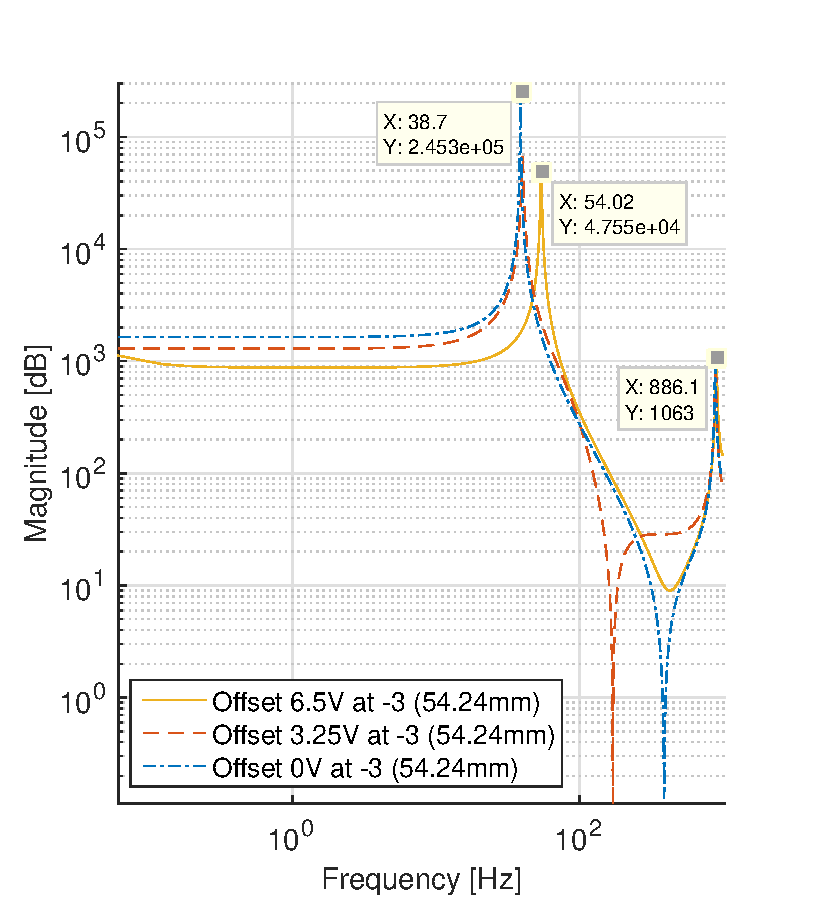
\includegraphics[width=0.4\textwidth]{../fig/matlab/modelcomparison_diffvolt2.eps}}
    \qquad
    \subfloat[][\label{fig:different_lin_pos}Model at different linear positions]{
    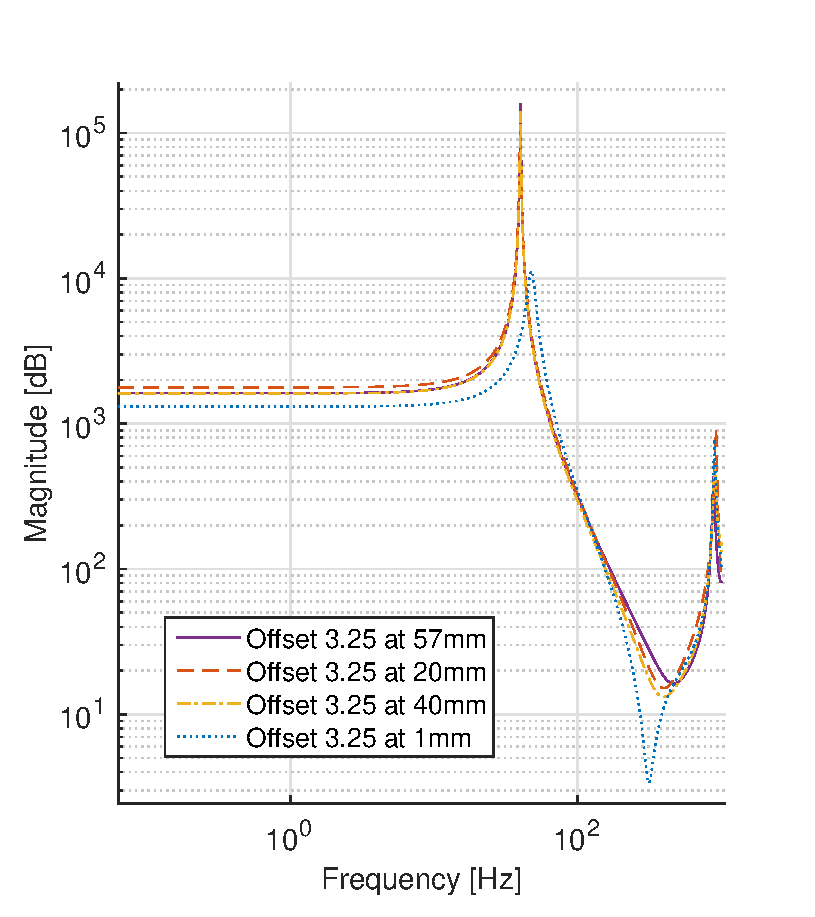
\includegraphics[width=0.4\textwidth]{../fig/matlab/modelcomparison2.eps}}
    %\caption{\label{fig:different_lin_angle} Identified models with different rotational positions (linear axis in 54.24 mm) is shown in (a) and with different linear axis positions (rotational position corresponding to 3.25 V) is shown in (b).}
  \end{figure}
\end{frame}

\begin{frame}{Present Control Approach}
  \begin{itemize}
    \item \alert{Hammerstein structure} - Model the rotational stage
    \item \alert{Hysteresis effect} - Modeled by a Maxwell slip model
    \item \alert{Creep effect} - Efficiently eliminated in closed loop
  \end{itemize}

  \begin{figure}[h]
    \centering %crop: left bottom right top
    \includegraphics[width=0.55\textwidth, trim=8cm 8cm 7.73cm 8cm, clip=true]{../fig/matlab/hammerstein}
    %\caption{\label{fig:hammerstein}Block diagram of a Hammerstein structure, consisting of two blocks in series, modeling the static hysteresis and the linear dynamics, respectively.}
  \end{figure}
  \vspace{-1cm}

  \begin{figure}[h]
    \centering %crop: left bottom right top
    \subfloat[][Hysteresis]{
    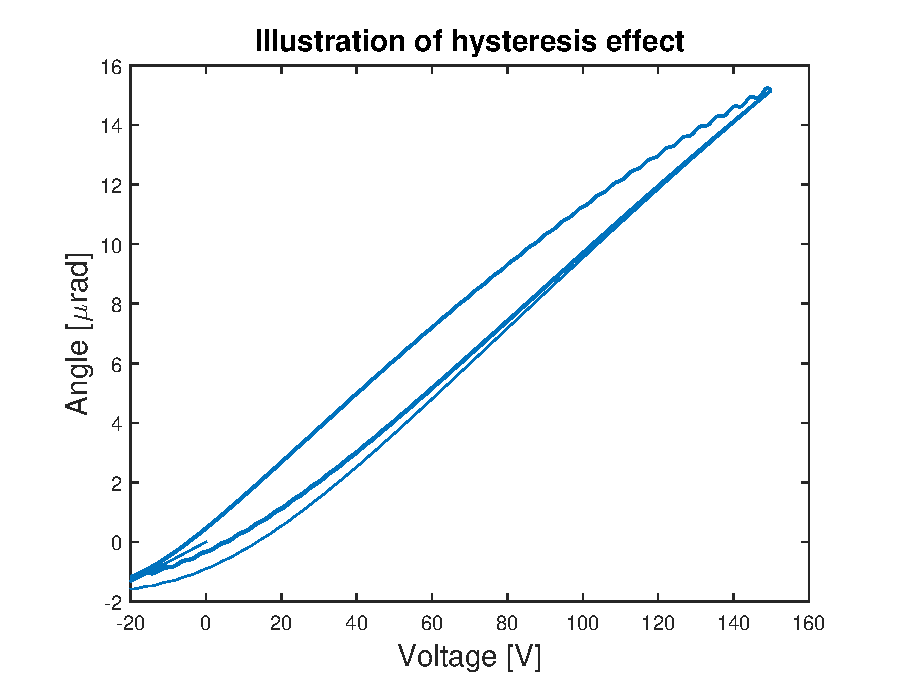
\includegraphics[width=0.27\textwidth]{../fig/matlab/hysteresis.eps}}
    \qquad
    \subfloat[][Creep]{
    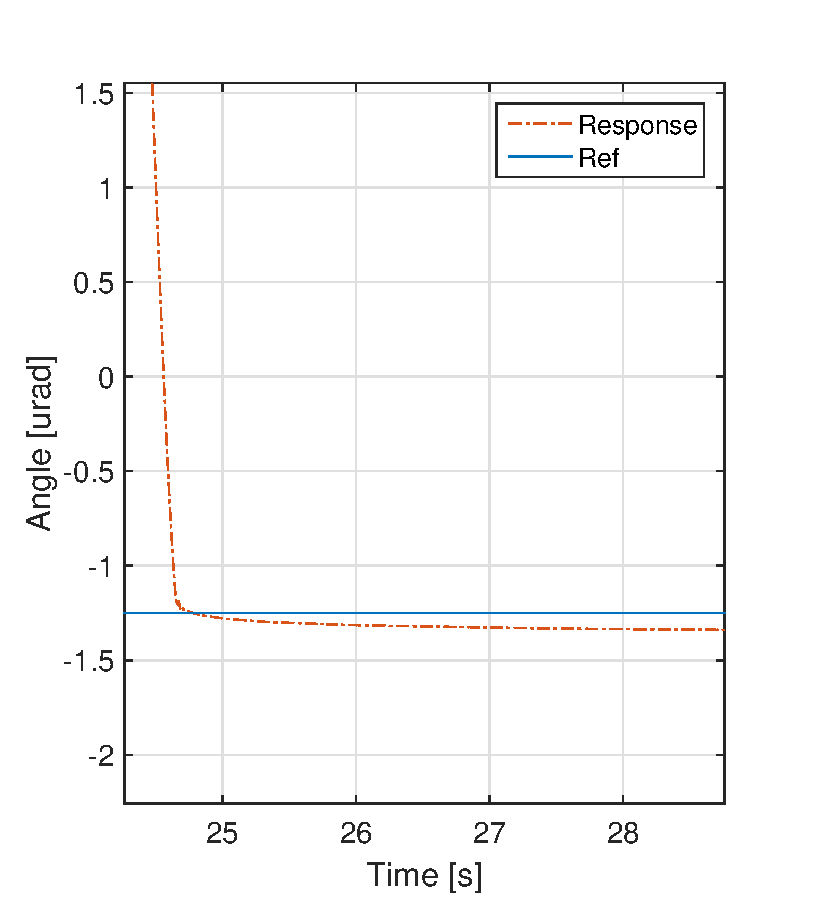
\includegraphics[width=0.27\textwidth]{../fig/matlab/creep.eps}}
    \qquad
    \subfloat[][Linear Model]{
    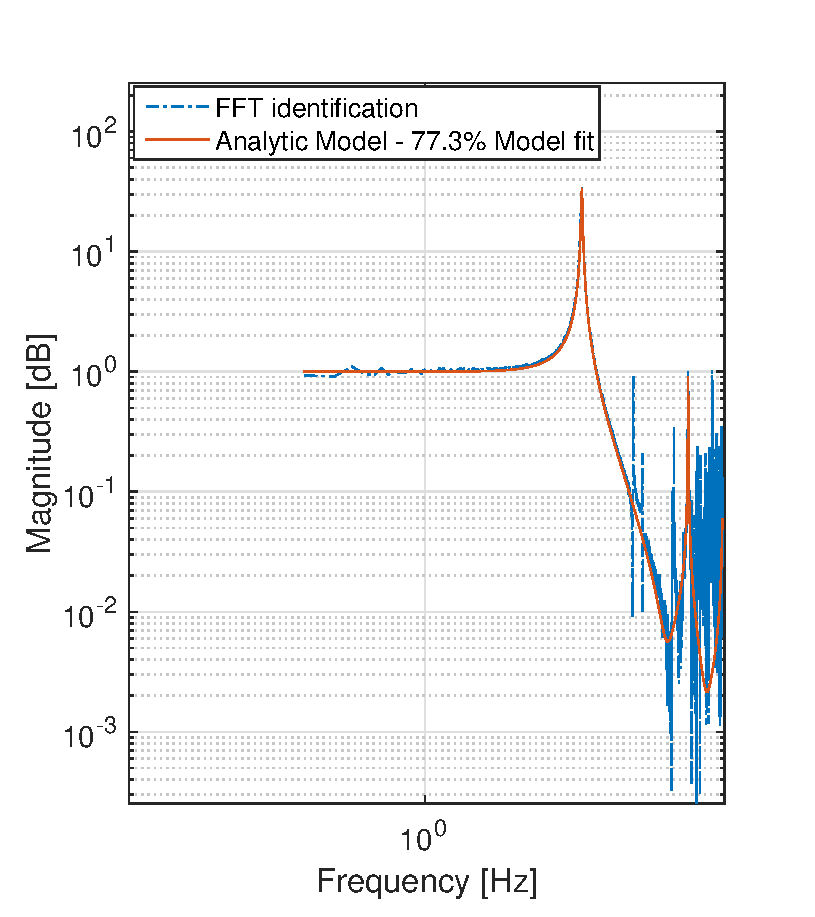
\includegraphics[width=0.27\textwidth]{../fig/matlab/model_long.eps}}
  \end{figure}
\end{frame}

\begin{frame}{Present Control Approach}
  2-DOF structure, feedback and prefilter.
  C is a series combination of:
  \begin{itemize}
    \item  \alert{PID} - for stablity
    \item  \alert{Notch filter} - to cancel high frequency oscillations
    \item  \alert{Lead filter} - to increase the phase margin
    \item \alert{Prefilter} - to increase closed loop bandwidth
  \end{itemize}

  \begin{figure}[h!]
    \centering %crop: left bottom right top
    \includegraphics[width=0.95\textwidth, trim=4cm 4cm 2.1cm 10cm, clip=true]{../fig/matlab/present_controller}
    %\caption{\label{fig:present}Block diagram of the present control loop, including controller, prefilter and hysteresis compensator.}
  \end{figure}
\end{frame}

\section{Approaches and Simulation Results}

\begin{frame}{Model Reference Adaptive Controller}
  \alert{Idea}: Adapt to model changes and compensate for nonlinear effects.
  \begin{itemize}
    \item Uses a reference model to create the desired system response.
    \item Based on Lyapunov theory
    \item Sufficient with a low order model
    \item Nonlinear effects is seen as lumped perturbations.
  \end{itemize}
  System model
    \begin{equation*}
      \label{eq:sysmodel}
      \ddot{x}(t) + \alpha_1\dot{x}(t) +  \alpha_0x(t) = \beta_0u(t) + f(t)
    \end{equation*}
  Reference model
    \begin{equation*}
      \label{eq:refmodel}
      \ddot{x}_m(t) + a_1\dot{x}_m(t) +  a_0x_m(t) = b_0u_d(t)
    \end{equation*}
  Final control law
    \begin{equation*}
        \label{eq:adaplawsfinal}
      u(t) = k_0u_d(t) + (k_1 + k_3\alpha_0)x(t) +  (k_2 + k_3\alpha_1)\dot{x}(t) + k_3\ddot{x}(t) - k_3\beta_0u(t-T_s)
    \end{equation*}
\end{frame}

\begin{frame}{Model Reference Adaptive Controller}
  \begin{figure}[h]
    \centering %crop: left bottom right top
    \includegraphics[width=0.75\textwidth, trim=5cm 0cm 3.8cm 0cm, clip=true]{../fig/matlab/adaptive_scheme}
    \caption{\label{fig:adaptive}Block diagram of the adaptive controller}
  \end{figure}
\end{frame}

\begin{frame}{Model Reference Adaptive Controller}
  Periodic response with model parameter drift increased linearly from $t=$ 7 s to $t=$ 9 s.
  \begin{figure}[h!]
    \centering %crop: left bottom right top
    \subfloat[][\label{fig:modeldriftresponse}Periodic response]{
    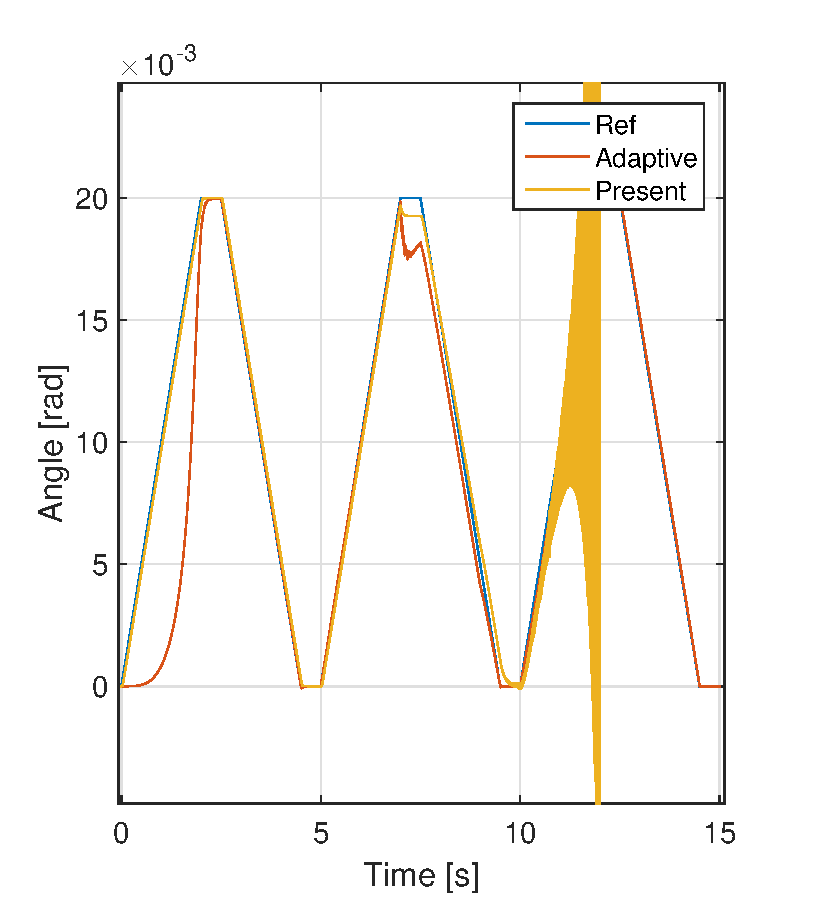
\includegraphics[width=0.4\textwidth, trim=0cm 0cm 1cm 0cm, clip=true]{../fig/matlab/driftofmodelparameterover2s.eps}}
    \qquad
    \subfloat[][\label{fig:modeldriftbode}Model change]{
    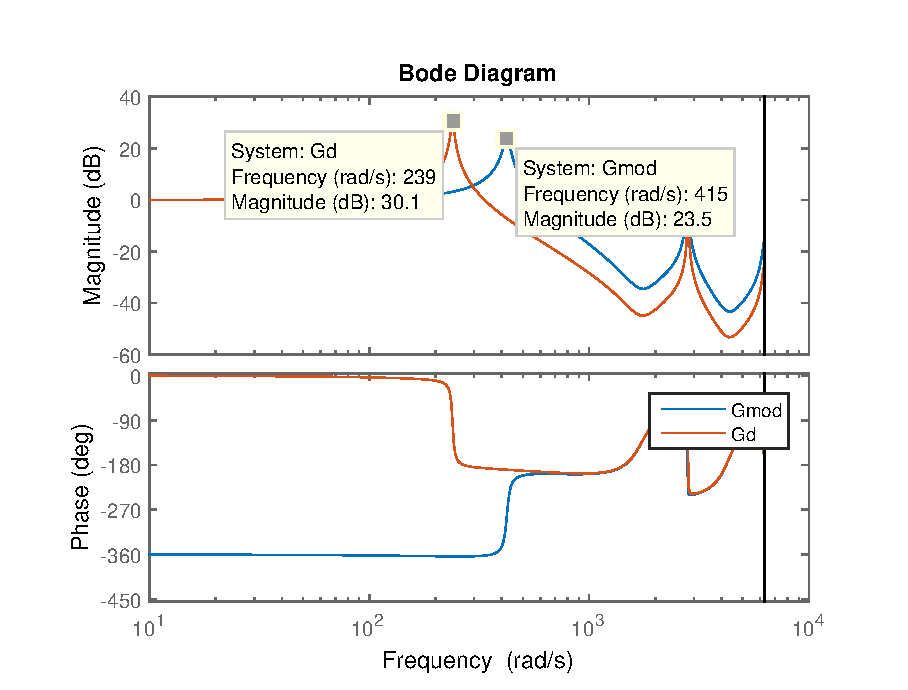
\includegraphics[width=0.42\textwidth, trim=0cm 0cm 0.7cm 0cm, clip=true]{../fig/matlab/bode_drift_pole.eps}}
  \end{figure}
\end{frame}

\begin{frame}{Integral Resonance Control}
  \alert{Idea}: Increase the yaw angle tracking accuracy.
  \begin{itemize}
    \item Uses a constant negative feed forward to damp out the first resonance peak
    \item Integral controller is used for inner loop stability
    \item C1 is designed for reference tracking and attenuating high frequency components
  \end{itemize}
  \vspace{-1cm}
  \begin{figure}[h!]
    \centering %crop: left bottom right top
    \subfloat[][]{
    \includegraphics[width=0.5\textwidth, trim=5.5cm 4cm 5.1cm 9.5cm, clip=true]{../fig/matlab/irc}} \\ \vspace{-1cm}
    \subfloat[][]{
    \includegraphics[width=0.7\textwidth, trim=4cm 5cm 3.6cm 9.5cm, clip=true]{../fig/matlab/irc_int}}
  \end{figure}
\end{frame}

\begin{frame}{Integral Resonance Control}
  \begin{itemize}
    \item Effect of IRC-damping.
    \item Increased closed loop bandwidth from 11 Hz to 73 Hz implying in a better tracking performance.
  \end{itemize}
  \vspace{-1cm}
  \begin{figure}[h!]
    \centering %crop: left bottom right top
    \subfloat[][IRC-damping]{
    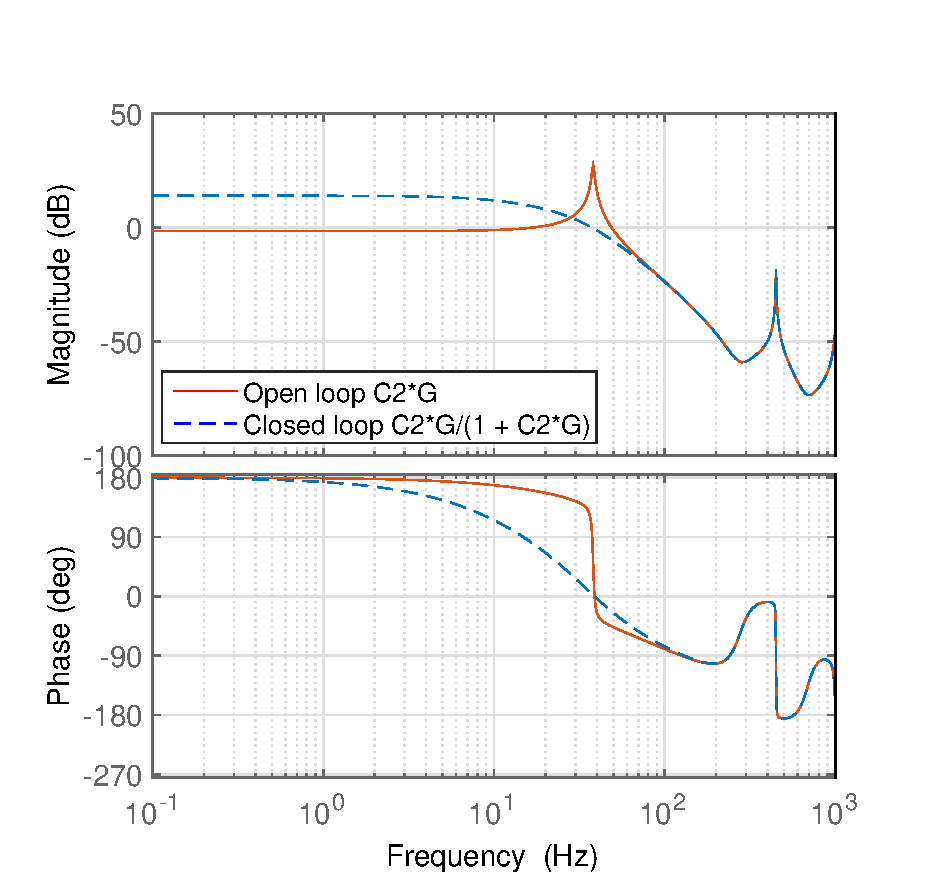
\includegraphics[width=0.5\textwidth]{../fig/matlab/bodedamped2}}
    \subfloat[][Closed loop bandwidth]{
    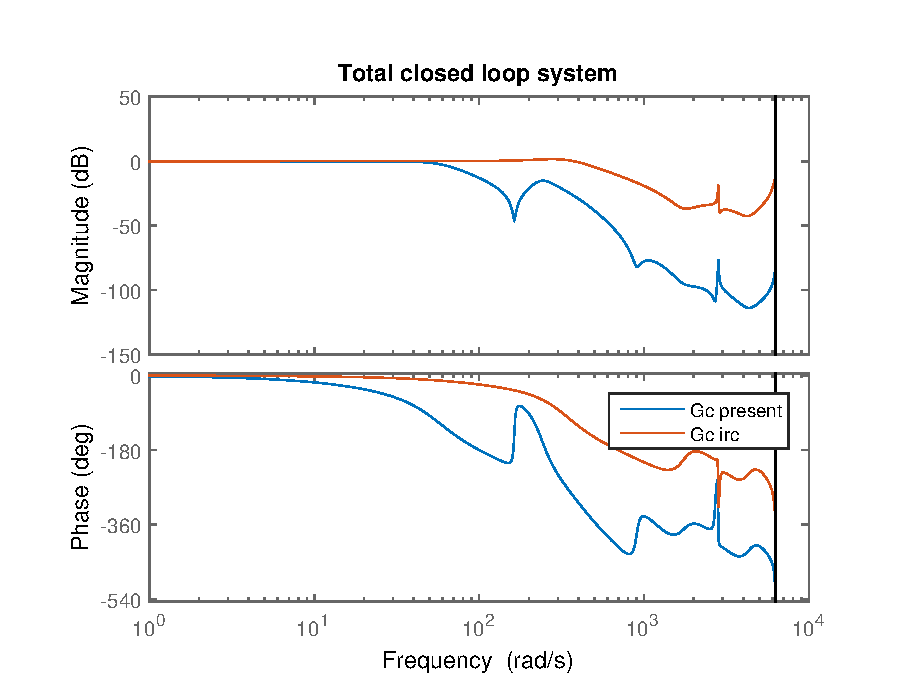
\includegraphics[width=0.5\textwidth]{../fig/matlab/totalclosedloop.eps}}
  \end{figure}
\end{frame}

\begin{frame}{Tracking performance comparison}
  Tracking error from periodic input with model parameter drift increased linearly from $t=$ 5 s to $t=$ 7 s.
  \\ {\color{white} -} \\
  \vspace{-1cm}
  \begin{figure}[h!]
    \centering %crop: left bottom right top
    \subfloat[][\label{fig:modelerrorbode}Model change]{
    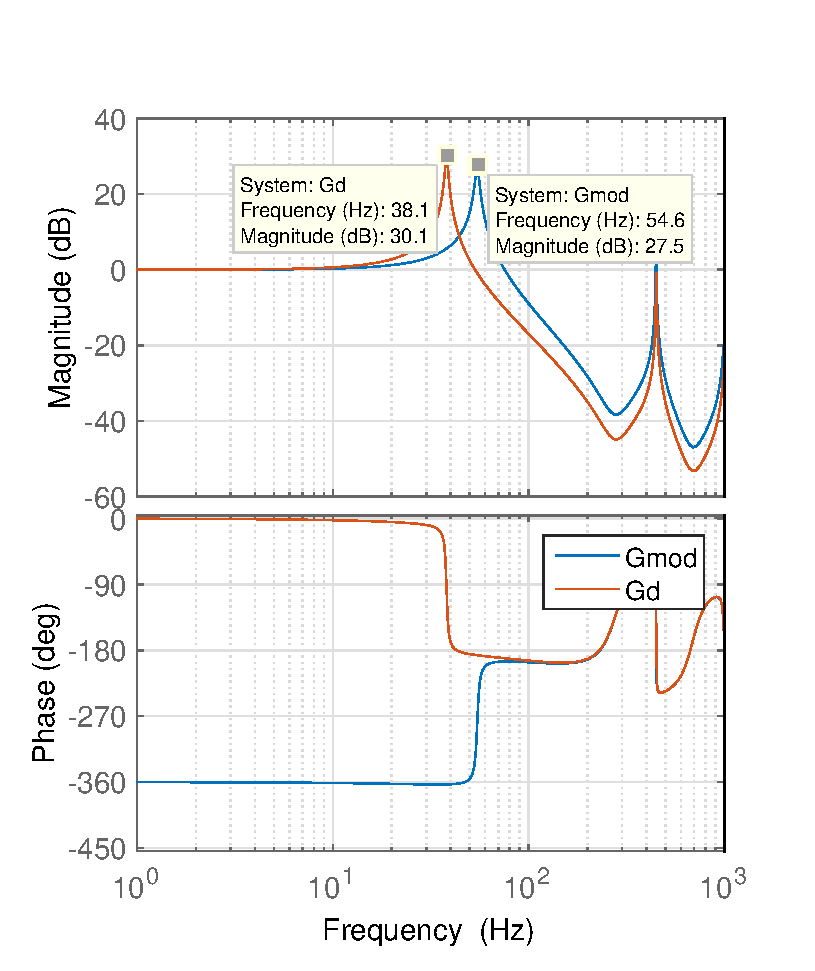
\includegraphics[width=0.47\textwidth, trim=0cm 0cm 0.7cm 0cm, clip=true]{../fig/matlab/bode_modelerror_pole.eps}}
    \qquad
    \subfloat[][\label{fig:irc_dist_model_drift}Tracking error]{
    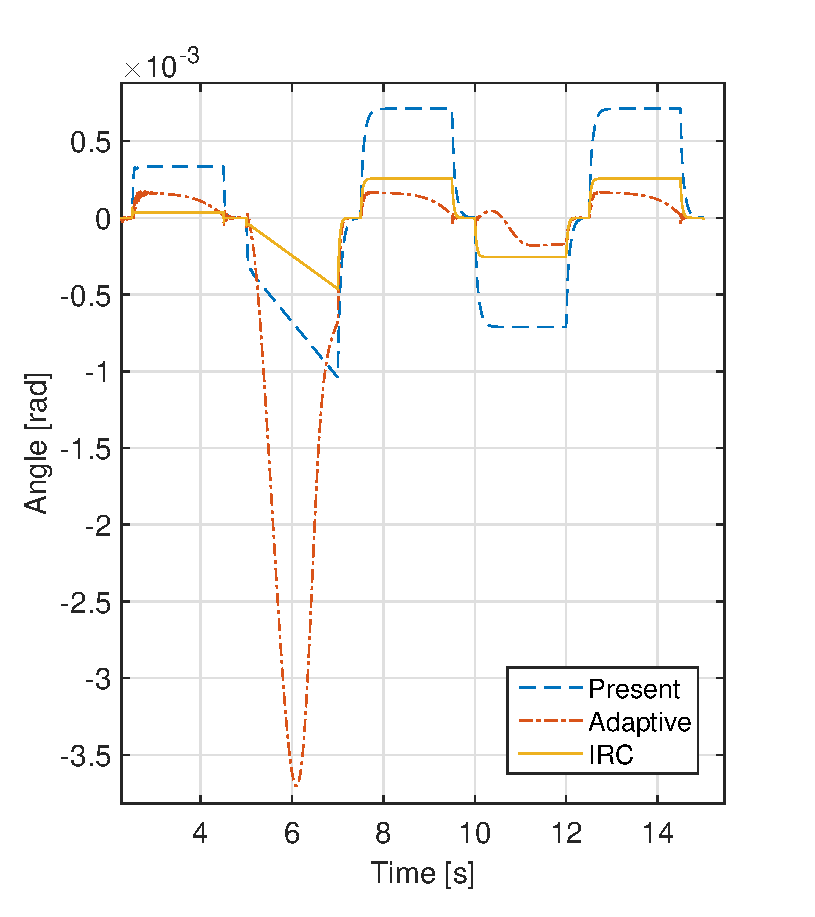
\includegraphics[width=0.43\textwidth, trim=0cm 0cm 1cm 0cm, clip=true]{../fig/matlab/tracking_error_lowf_model_change}}
  \end{figure}
\end{frame}

\begin{frame}{Harmonic Cancellation}
  \alert{Idea}: Cancel out specific disturbances coming from the environment in the tunnel or the linear stage movement.
  \begin{itemize}
    \item Feedforward Disturbance Cancellation
    \item Cancellation with Internal Model Principle
    \item Repetitive Feedforward Disturbance Cancellation
  \end{itemize}
  \alert{Repetitive Feedforward Disturbance Cancellation}: Use an observer to estimate and cancel known disturbances without affecting the closed loop system.
  \begin{itemize}
    \item First introduced for the control of hard disks
    \item Feedforward switching mechanism with an observer
    \item Not affecting the closed loop system
  \end{itemize}
\end{frame}

\begin{frame}{Repetitive Feedforward Disturbance Cancellation}
The state space system and observer is given as
  \begin{subequations}
    \label{eq:sys12}
    \begin{alignat}{2}
      \label{eq:sys1}
      & \mathbf{\dot{x}}(t) = \mathbf{A_cx}(t) + \mathbf{B_c}\big(u(t) + d_o(t)\big) \\
      \label{eq:sys2}
      & y(t) = \mathbf{C_cx}(t) \\
      \label{eq:dist1}
      & \mathbf{\dot{x}}_d(t) = \mathbf{A_dx_d}(t) \\
      \label{eq:dist2}
      & d_o(t) = \mathbf{C_dx_d}(t)
    \end{alignat}
  \end{subequations}

  \begin{equation*}
    \label{eq:sinm}
    \frac{1}{w}\sin(wt)
    \implies
    \mathbf{A_d} =
      \begin{bmatrix}
         0 & 1\\[0.3em]
         -w^2 & 0
       \end{bmatrix}
       \qquad
    \mathbf{C_d} =
      \begin{bmatrix}
          1 & 0\\
      \end{bmatrix}
  \end{equation*}

  \begin{equation*}
    \label{eq:obs}
    \mathbf{\hat{x}}[n + 1] = \mathbf{A\hat{x}}[n] + \mathbf{B}u[n] + \mathbf{K}(\mathbf{y}[n] - \mathbf{C\hat{x}}[n])
  \end{equation*}

  \begin{equation*}
    \label{eq:augumented}
    \mathbf{A} =
      \begin{bmatrix}
         \mathbf{A_{zs}} & \mathbf{C_{zd}B_{zs}}\\[0.3em]
         \mathbf{0} & \mathbf{A_{zd}}\\
       \end{bmatrix}
       \qquad
    \mathbf{B} =
      \begin{bmatrix}
          \mathbf{B_{zs}}\\
          \mathbf{0}
      \end{bmatrix}
       \qquad
    \mathbf{C} =
      \begin{bmatrix}
          \mathbf{C_{zs}} & \mathbf{0}\\
      \end{bmatrix}
  \end{equation*}
\end{frame}

\begin{frame}{Repetitive Feedforward Disturbance Cancellation}
  \begin{figure}[h]
    \centering %crop: left bottom right top
    \includegraphics[width=0.7\textwidth, trim=6cm 5.5cm 5.2cm 5.5cm, clip=true]{../fig/matlab/ffrep}
  \end{figure}
  \vspace{-1cm}
  \begin{figure}[h!]
    \centering
    \subfloat[][]{
    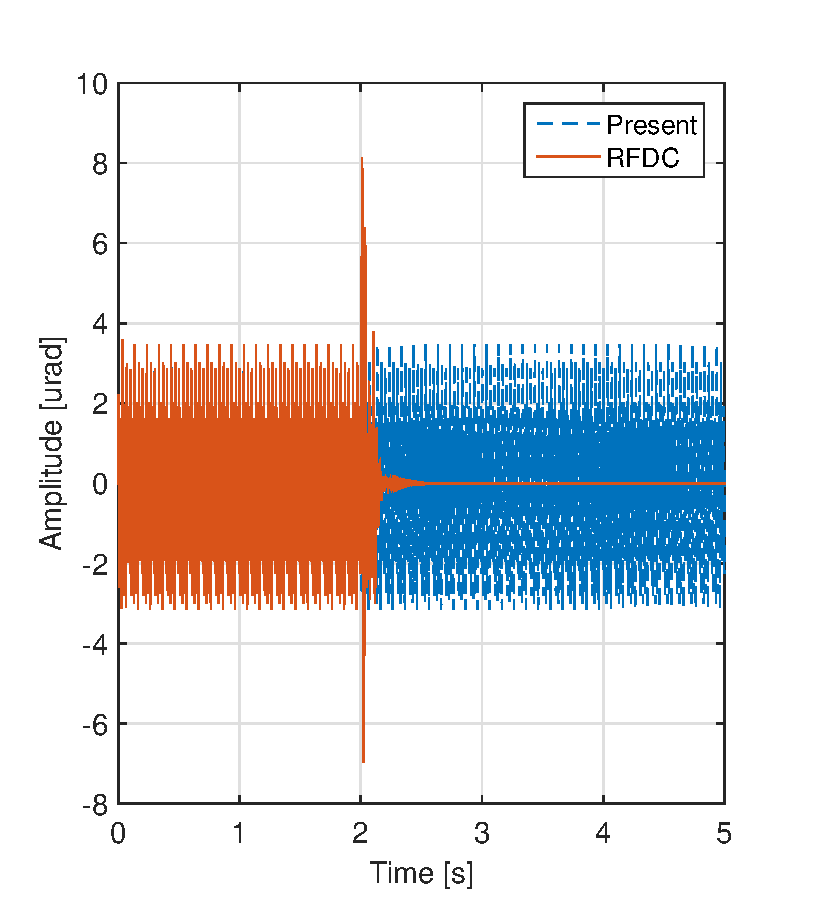
\includegraphics[width=0.3\textwidth]{../fig/matlab/3_dist.eps}}
    \subfloat[][]{
    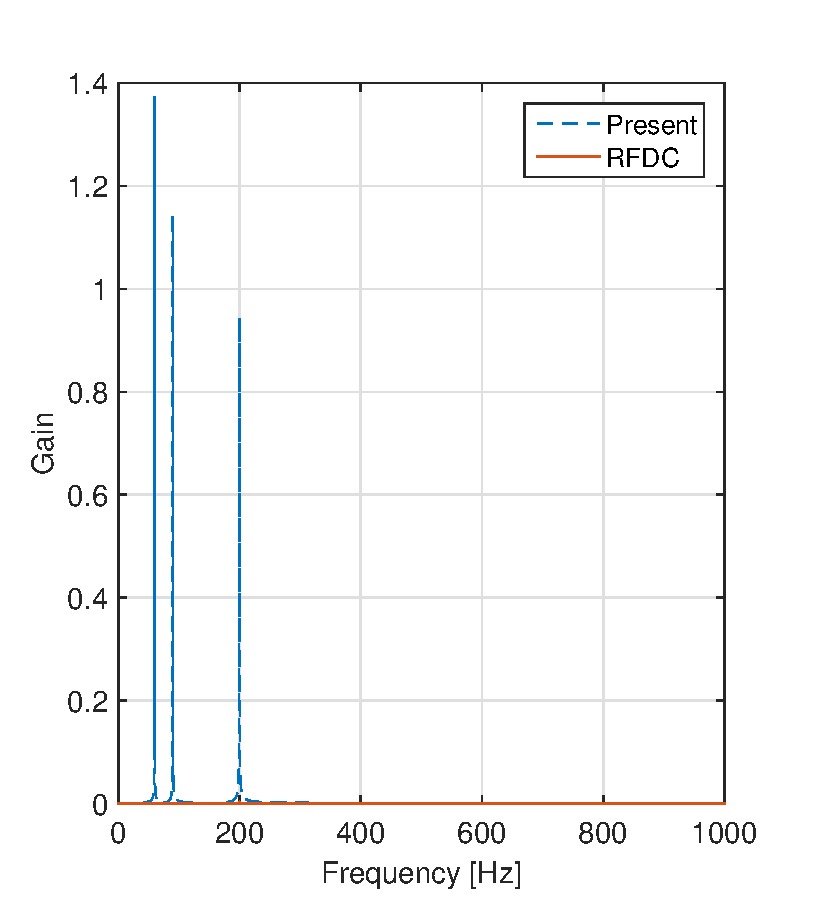
\includegraphics[width=0.3\textwidth]{../fig/matlab/3_dist_fft.eps}}
  \end{figure}
\end{frame}

\section{Implementation}

\begin{frame}{Setup}
  \begin{itemize}
    \item Implementation in LabVIEW
    \item Deployed on a National Instruments PXI (2kHz)
    \item Shaker
  \end{itemize}
  \begin{figure}[h]
    \centering
    \subfloat[][Shaker]{
    \includegraphics[width=0.27\textwidth]{../fig/shaker}}
    \subfloat[][GUI]{
    \includegraphics[width=0.59\textwidth]{../fig/HC_gui}}
  \end{figure}
\end{frame}

\begin{frame}{Cancellation verification}
  \begin{itemize}
    \item \alert(Single disturbance) 80 Hz (76\%)
    \item \alert(Multiple disturbances) 50Hz (75\%) 80Hz (66\%)
  \end{itemize}
  \vspace{-1cm}
  \begin{figure}[h]
    \centering
    \subfloat[][]{
    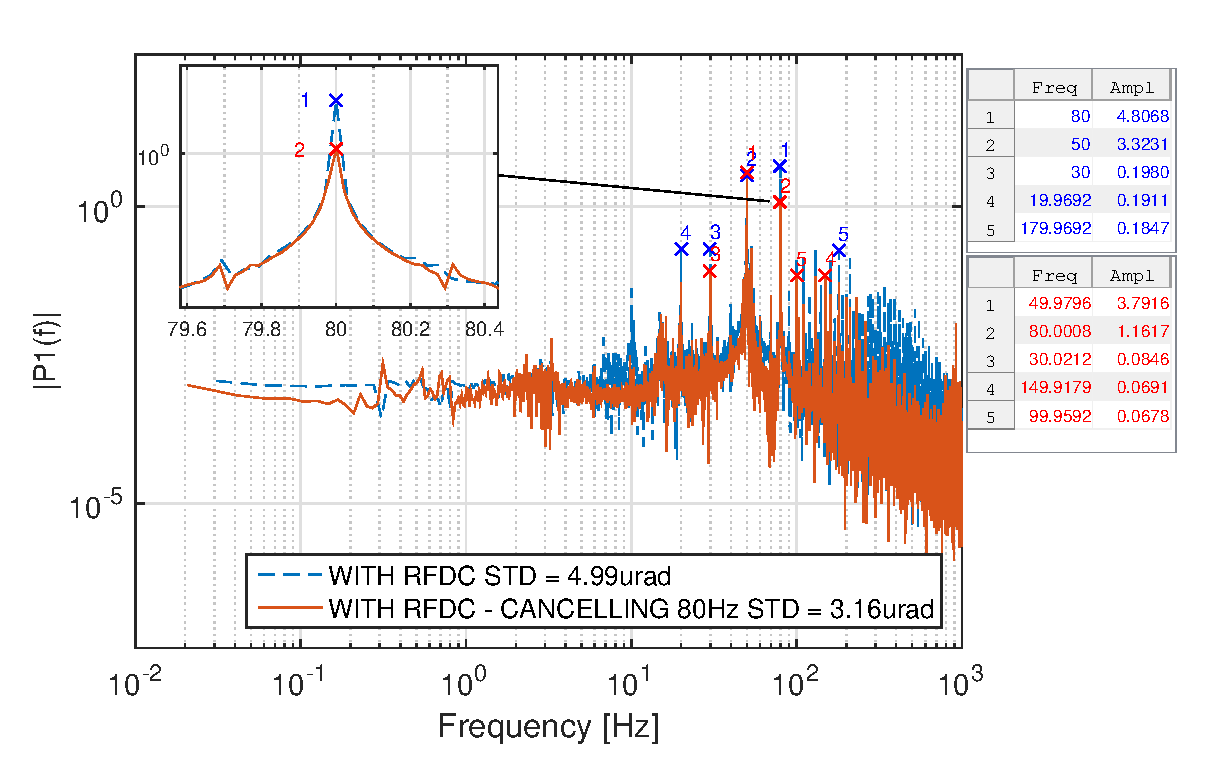
\includegraphics[width=0.5\textwidth]{../fig/matlab/fft_closedloop_ext_disturbance_80Hz_with_zoom_2}}
    \subfloat[][]{
    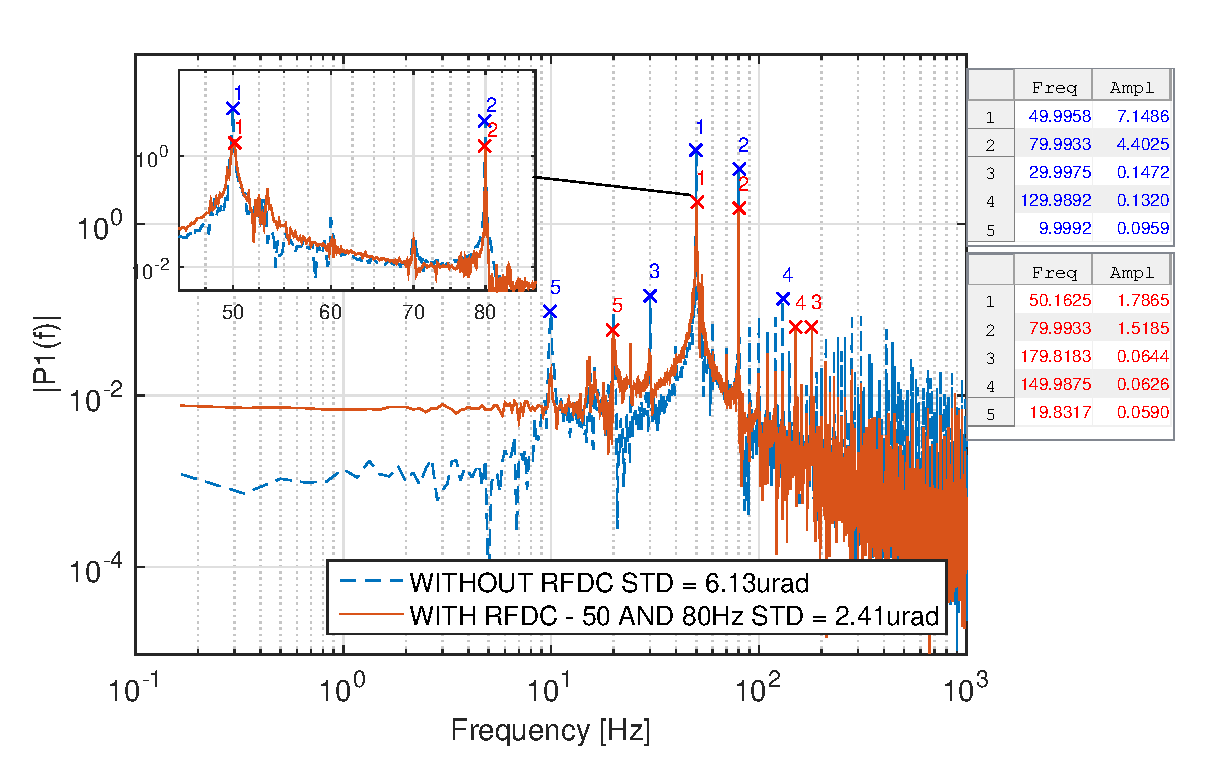
\includegraphics[width=0.5\textwidth]{../fig/matlab/mult_50_80_closed_loop}}
    %\caption{\label{fig:mult5080} Multiple cancellation in closed loop of the 50 and the 80 Hz component. The plot is based on a 10 s long acquisition.}
  \end{figure}
\end{frame}

\begin{frame}{Beat effect}
  Cancellation performance varies, esp. for cancellation close to the resonance.

  \vspace{-1cm}
  \begin{figure}[h!]
    \centering %crop: left bottom right top
    \subfloat[][]{
    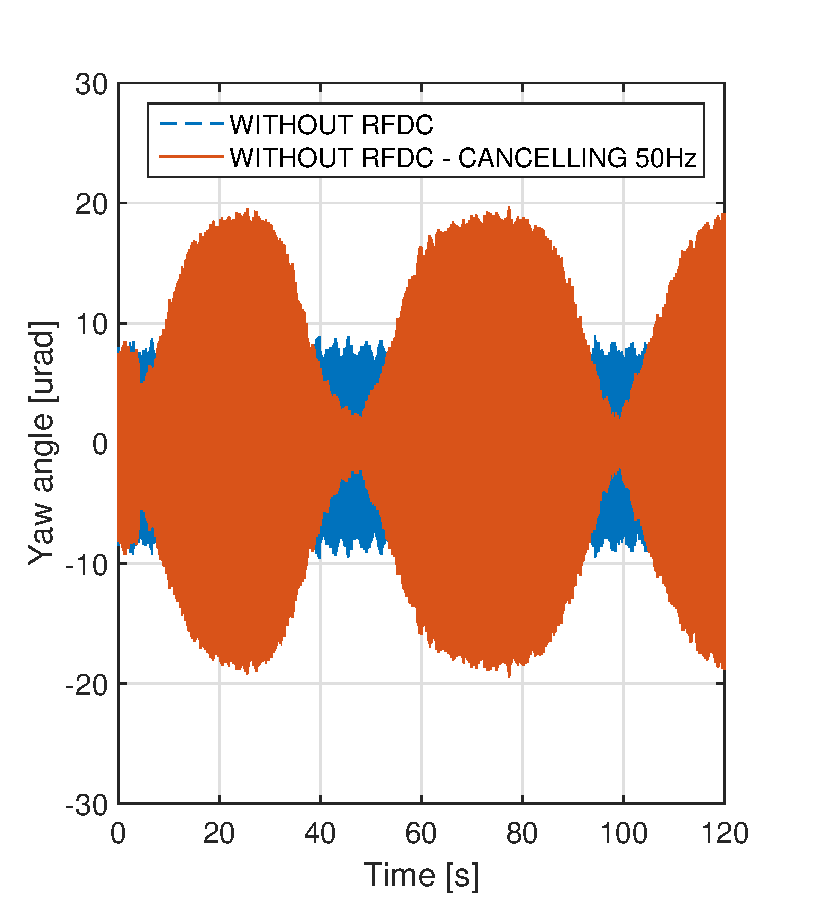
\includegraphics[width=0.3\textwidth]{../fig/matlab/beat_effect_yl}}
    \subfloat[][]{
    \includegraphics[width=0.3\textwidth]{../fig/matlab/beat_effect}} \\ {\color{white} -} \\ \vspace{-1cm}
    \subfloat[][]{
    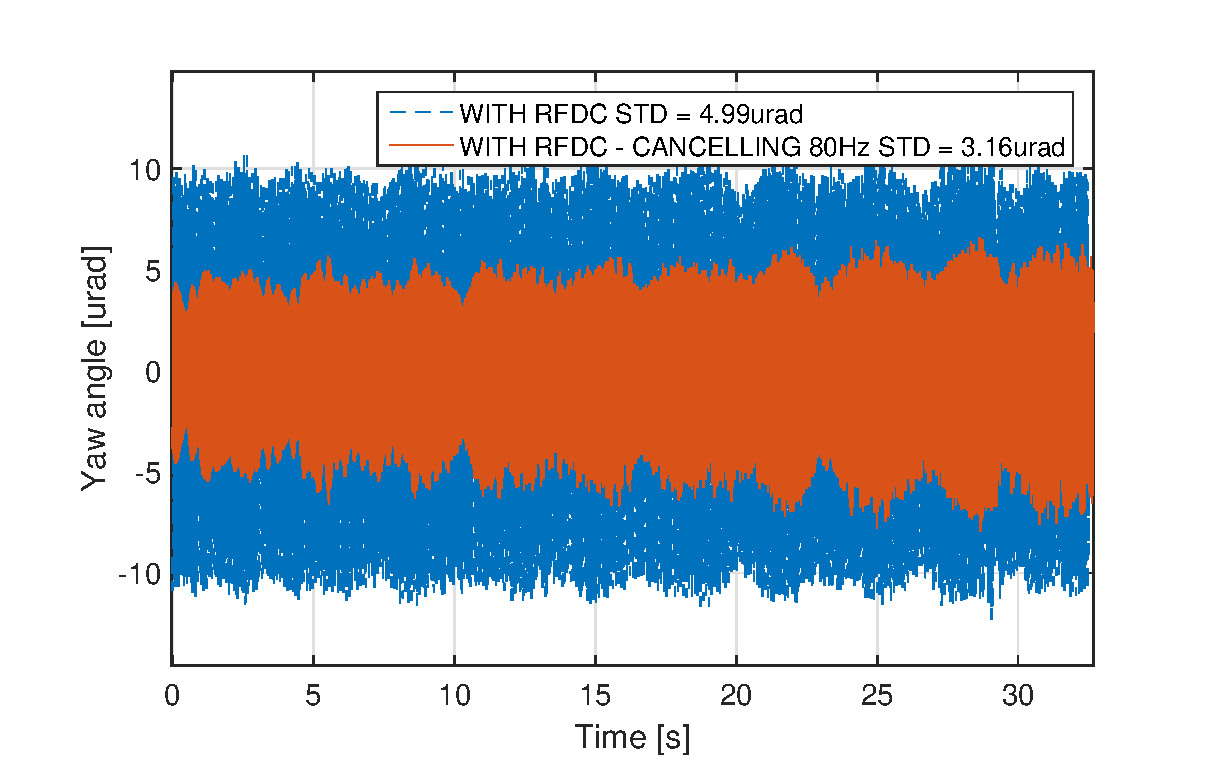
\includegraphics[width=0.5\textwidth]{../fig/matlab/yl_closedloop_ext_disturbance_80Hz_2}}
  \end{figure}
\end{frame}

\section{Conclusion}

\begin{frame}{Summary of Findings}
  IRC
  \begin{itemize}
    \item  Can be used to efficiently increase the closed loop bandwidth
    \item  No direct information of the first resonance peak
    \item  Tradeoff: Tracking performance - Controller robustness
  \end{itemize}
  MRACPE
  \begin{itemize}
    \item Can be used to adapt to large model changes and thereby prevent instability
    \item Tradeoff: Adaption time - Stability
  \end{itemize}
  RFDC
  \begin{itemize}
    \item Can be used to efficiently damp out known harmonic oscillations (even outside the closed loop bandwidth)
    \item Beat effect. Less obvious for generated disturbance
    \item Tradeoff: Convergence time - Cancellation effectiveness
  \end{itemize}
\end{frame}

\begin{frame}{Future Work}
  IRC + Adaptive + RFDC
  \begin{itemize}
    \item Combination of two or three approaches
    \item Increasing tracking performance
    \item Adaptive to long term changes such as temperature and radiation
  \end{itemize}
  Improvement of the RFDC
  \begin{itemize}
    \item More investigation in the cancellation performance.
    \item Beat effect solutions:
    \begin{itemize}
      \item Increase observation time
      \item Use a few elements to synchronize the replicated signal.
    \end{itemize}
  \end{itemize}
  Improvement of the mechanical design
  \begin{itemize}
    \item CERN is now developing a new rotational stage
    \item Applies the force directly to the rotational head
    \item More stiff $\implies$ higher bandwidth, easier to design a sufficient controller
  \end{itemize}
\end{frame}


%\section{Questions?}[standout]
\begin{frame}[standout]
   Thank you!
\end{frame}

\appendix

\begin{frame}{Model Reference Adaptive Controller}
  \begin{equation*}
    \label{eq:stateerror}
    e(t) = x(t) - x_m(t)
  \end{equation*}

  \begin{equation*}
    \ddot{e}(t) + a_1\dot{e}(t) + a_0\dot{e}(t) =  (a_1-\alpha_1)\dot{x}(t) + (a_0-\alpha_0)x(t) - b_0u_d(t) - \beta_0u(t) + \hat{f}(t)
  \end{equation*}
  \begin{equation*}
    \label{eq:stateSpaceError}
    \mathbf{\dot{E} = AE} + \beta_0\mathbf{B}u + \Delta
  \end{equation*}
  where
  \begin{equation*}
    \label{eq:matrices}
    \mathbf{E} =
      \begin{bmatrix}
         e\\[0.3em]
         \dot{e}
       \end{bmatrix},
    \mathbf{A} =
      \begin{bmatrix}
         0 & 1\\[0.3em]
         -a_0 & -a_1
       \end{bmatrix},
    \mathbf{B} =
      \begin{bmatrix}
          0\\[0.3em]
          1
      \end{bmatrix},
      \mathbf{\Delta} =
        \begin{bmatrix}
            0\\[0.3em]
            \delta
        \end{bmatrix}
  \end{equation*}
  with $\delta = (a_1-\alpha_1)\dot{x}(t) + (a_0-\alpha_0)x(t) - b_0u_d(t) + \hat{f}(t)$.

  If all eigenvalues of $\mathbf{A}$ have negative real parts, then $\mathbf{E}$ will tend to zero as  $t \to \infty$, i.e. the system is asymptotically stable. According to Lyapunov theory, for each positive-semidefinite matrix $\mathbf{Q}$ there exists one positive-semidefinite matrix $\mathbf{P}$ which solves \eqref{eq:lyap}.
\end{frame}

\begin{frame}{Model Reference Adaptive Controller}

  \begin{equation*}
    \label{eq:lyap}
    \mathbf{A^TP + PA = -Q}
  \end{equation*}

  With the auxiliary item $\hat{e} = \mathbf{E^TPB}$, the adaptive laws are given by

  \begin{equation*}
    \label{eq:adaplaws}
    u = k_0u_d + k_1x + k_2\dot{x} + k_3\hat{f}
  \end{equation*}
  where the control law parameters are calculated as outlined below.
  \begin{equation*}
    \label{eq:adaplaws1}
    \dot{k}_0 = -\eta_0\hat{e}u_d
  \end{equation*}
  \begin{equation*}
    \label{eq:adaplaws2}
    \dot{k}_1 = -\eta_1\hat{e}x
  \end{equation*}
  \begin{equation*}
    \label{eq:adaplaws3}
    \dot{k}_2 = -\eta_2\hat{e}\dot{x}
  \end{equation*}
  \begin{equation*}
    \label{eq:adaplaws4}
    \dot{k}_3 = -\eta_3\hat{e}\hat{f}
  \end{equation*}

  \begin{equation*}
      \label{eq:adaplawsfinal}
    u(t) = k_0u_d(t) + (k_1 + k_3\alpha_0)x(t) +  (k_2 + k_3\alpha_1)\dot{x}(t) + k_3\ddot{x}(t) - k_3\beta_0u(t-T_s)
  \end{equation*}
\end{frame}

\begin{frame}{Model Reference Adaptive Controller}
  Periodic response with model parameter drift increased linearly from $t=$ 5 s to $t=$ 7 s.
  \begin{figure}[h!]
    \centering %crop: left bottom right top
    \subfloat[][\label{fig:modelerrorresponse}Periodic response]{
    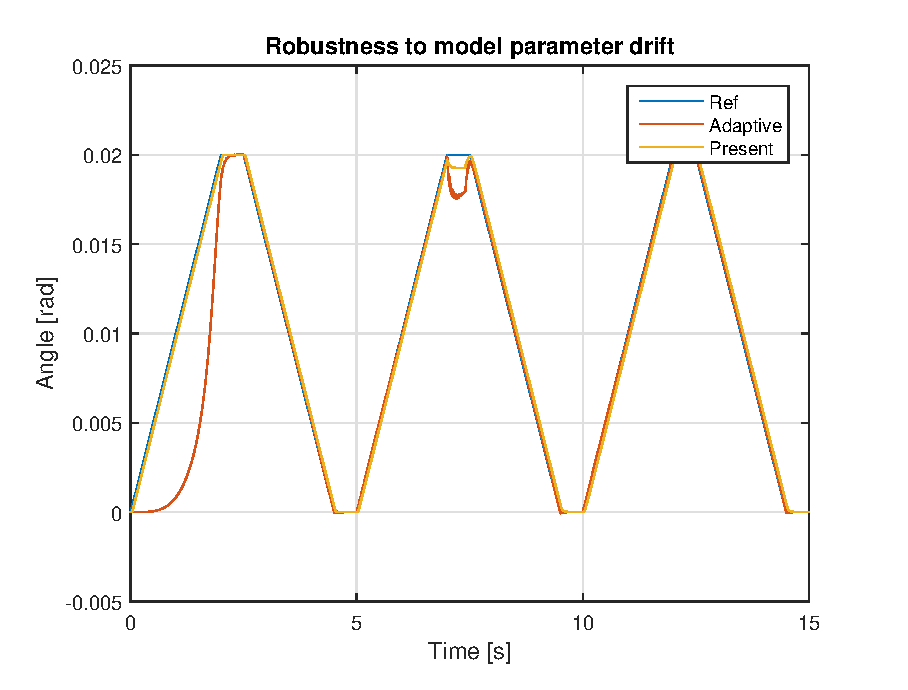
\includegraphics[width=0.4\textwidth, trim=0cm 0cm 1cm 0cm, clip=true]{../fig/matlab/modelerrorperiodic.eps}}
    \qquad
    \subfloat[][\label{fig:modelerrorbode}Model change]{
    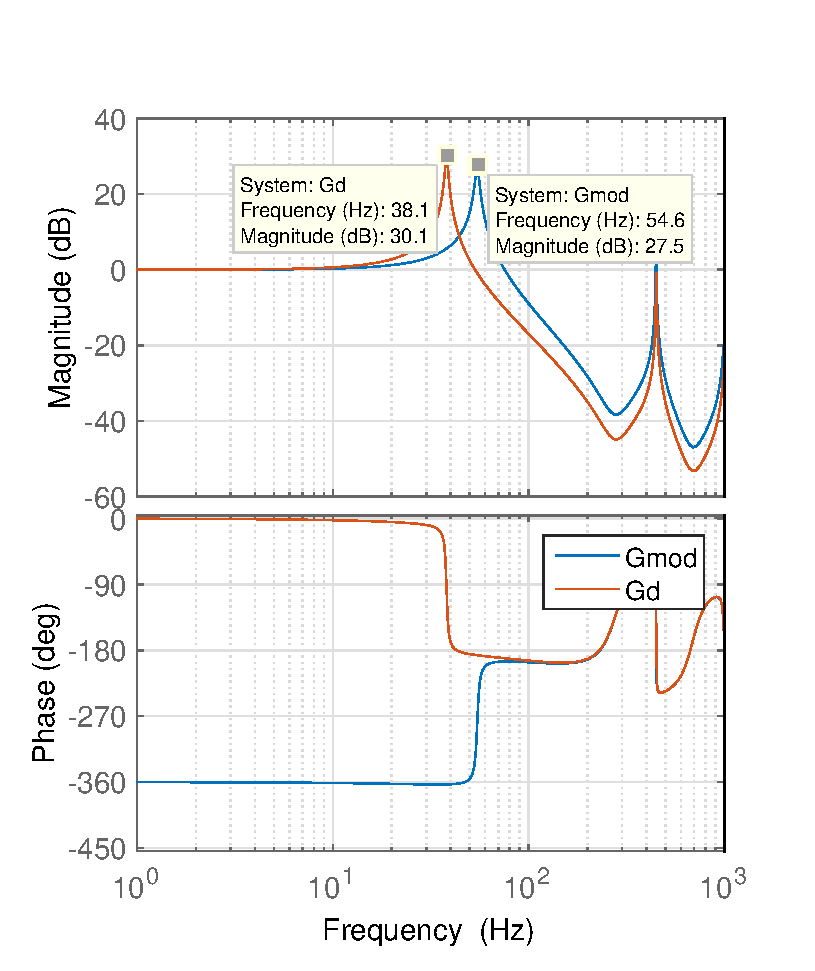
\includegraphics[width=0.42\textwidth, trim=0cm 0cm 0.7cm 0cm, clip=true]{../fig/matlab/bode_modelerror_pole.eps}}
  \end{figure}
\end{frame}

\begin{frame}{Model Reference Adaptive Controller}
  Tracking error
  \begin{figure}[h!]
    \centering
    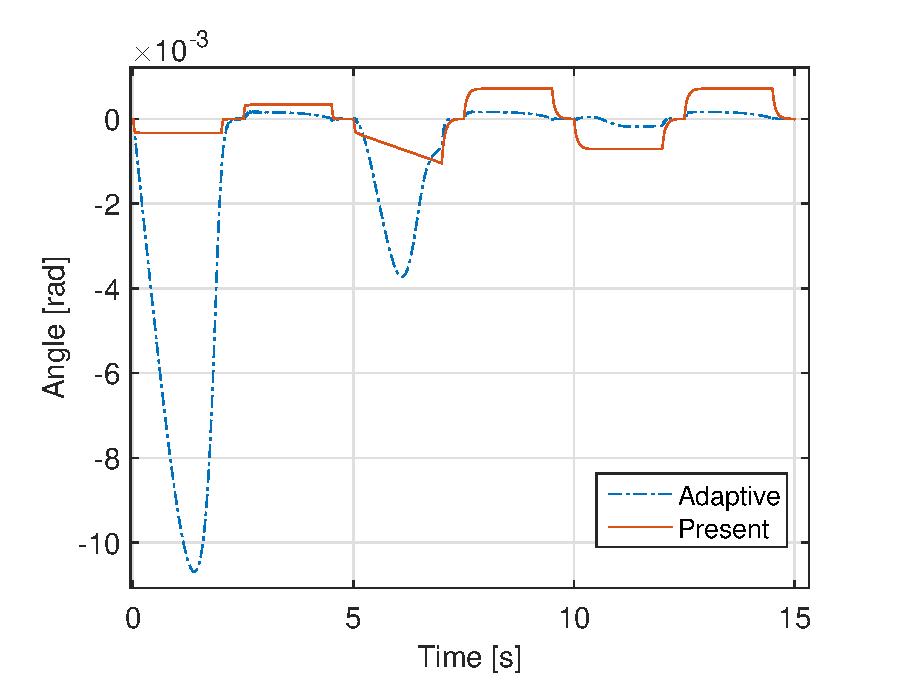
\includegraphics[width=0.7\textwidth]{../fig/matlab/modelerrorperiodic_trackingerror.eps}
    %\caption{\label{fig:modelerror_trackingerror} Tracking error}
  \end{figure}
\end{frame}

\begin{frame}{Feedforward Disturbance Cancellation}
  \alert{Idea}: Use a feedforward approach to cancel out known disturbances coming from the linear axis movement.
  \begin{itemize}
    \item Identify a static disturbance model
    \item Use the stepping signal as input to the model
    \item Disturbance must be measurable
  \end{itemize}
\end{frame}

\begin{frame}{Feedforward Disturbance Cancellation}
  \begin{figure}[h]
    \centering %crop: left bottom right top
    \includegraphics[width=0.8\textwidth, trim=8cm 4.5cm 5.97cm 8.5cm, clip=true]{../fig/matlab/ffdist}
    %\caption{\label{fig:ffdist}Block diagram of a control structure with feedforward from a known modeled disturbance.}
  \end{figure}
  \begin{equation*}
    \label{eq:ffdist}
    Y(s) = \frac{C(s)G(s)}{1+C(s)G(s)}R(s) + \frac{P_d(s) - K_f(s)G(s)}{1+C(s)G(s)}D_0(s)
  \end{equation*}
  Ideal choice: $K_f(s)=P_d(s)/G(s)$

   $K_f(s)$ not implementable (stable, proper and causal). $\implies$
   Approximate $G$.
\end{frame}

\begin{frame}{Feedforward Disturbance Cancellation}
  \begin{figure}[h!]
    \centering %crop: left bottom right top
    \subfloat[][\label{fig:stepin}Impulse used as input signal]{
    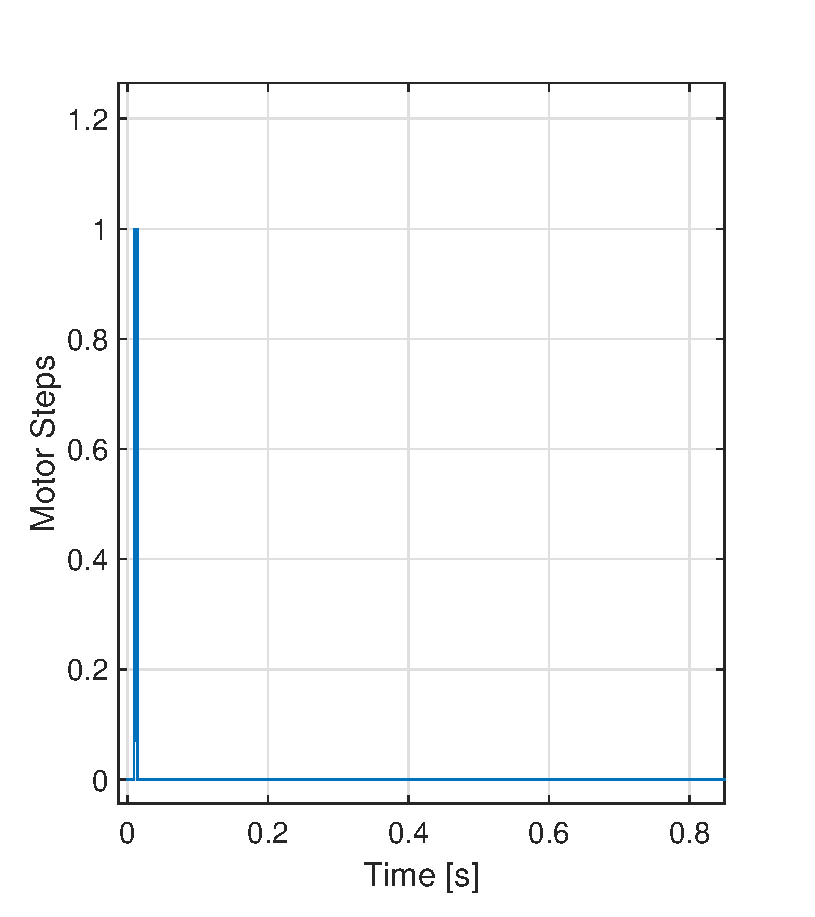
\includegraphics[width=0.43\textwidth, trim=0cm 0cm 1cm 0.8cm, clip=true]{../fig/matlab/ff_impulse.eps}}
    \qquad
    \subfloat[][\label{fig:stepout}Mean of impulse responses]{
    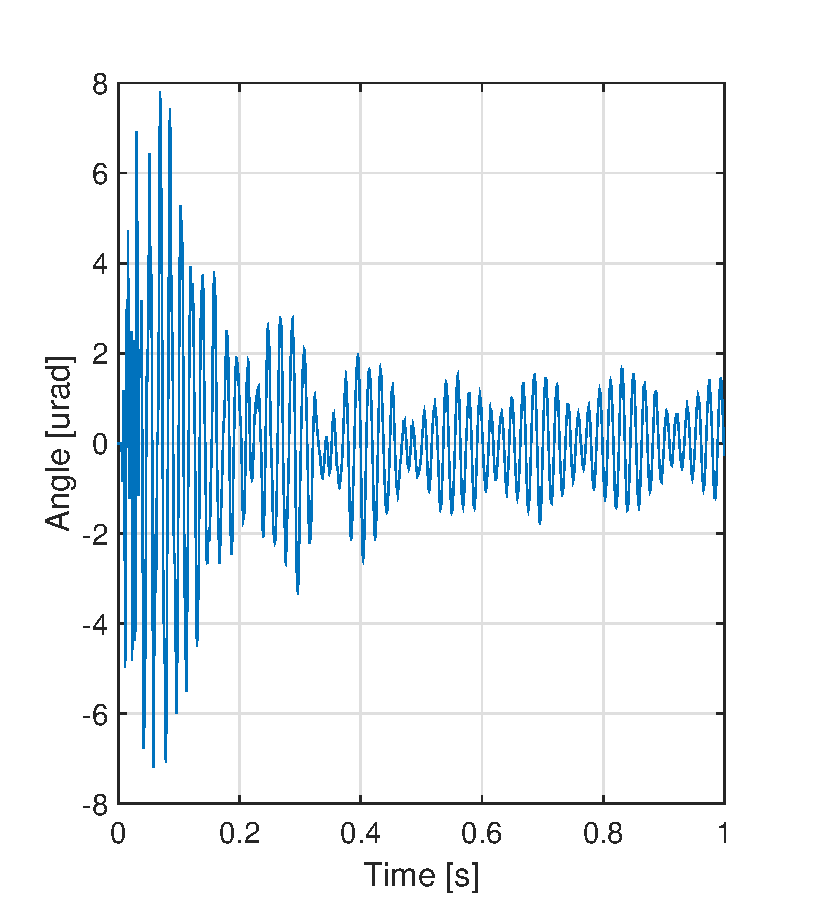
\includegraphics[ width=0.43\textwidth, trim=0cm 0cm 1cm 0.8cm, clip=true]{../fig/matlab/yaw_angle_mean_1_step_s.eps}}
    %\caption{\label{fig:stepinout} Input signal (a) and step response (b) used for modeling the disturbance. The step response was calculated by taking the mean of 50 time-synchronized acquired step responses at a movement of 1 step/s.}
  \end{figure}
\end{frame}

\begin{frame}{Feedforward Disturbance Cancellation}
  \begin{figure}[h!]
    \centering %crop: left bottom right top
    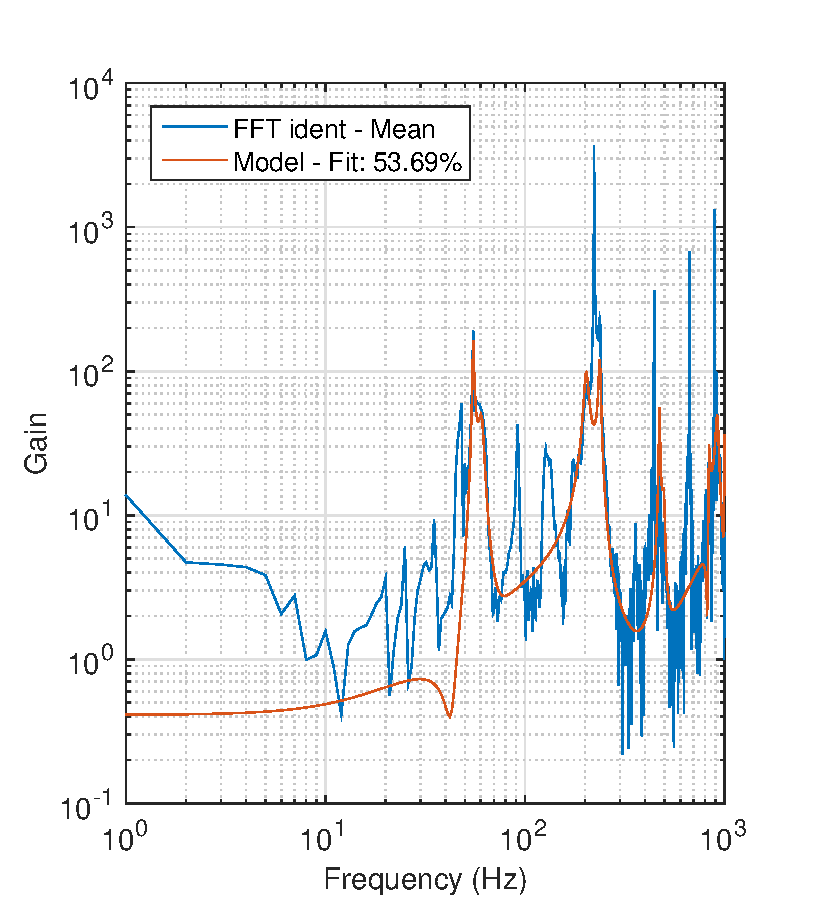
\includegraphics[width=0.6\textwidth,]{../fig/matlab/model_fit_1step_s.eps}
    %\caption{\label{fig:imp}Block diagram of the \abbrIMP control structure.}
  \end{figure}
\end{frame}

\begin{frame}{Feedforward Disturbance Cancellation}
  \begin{figure}[h!]
    \centering %crop: left bottom right top
    \subfloat[][Mean as disturbance]{
    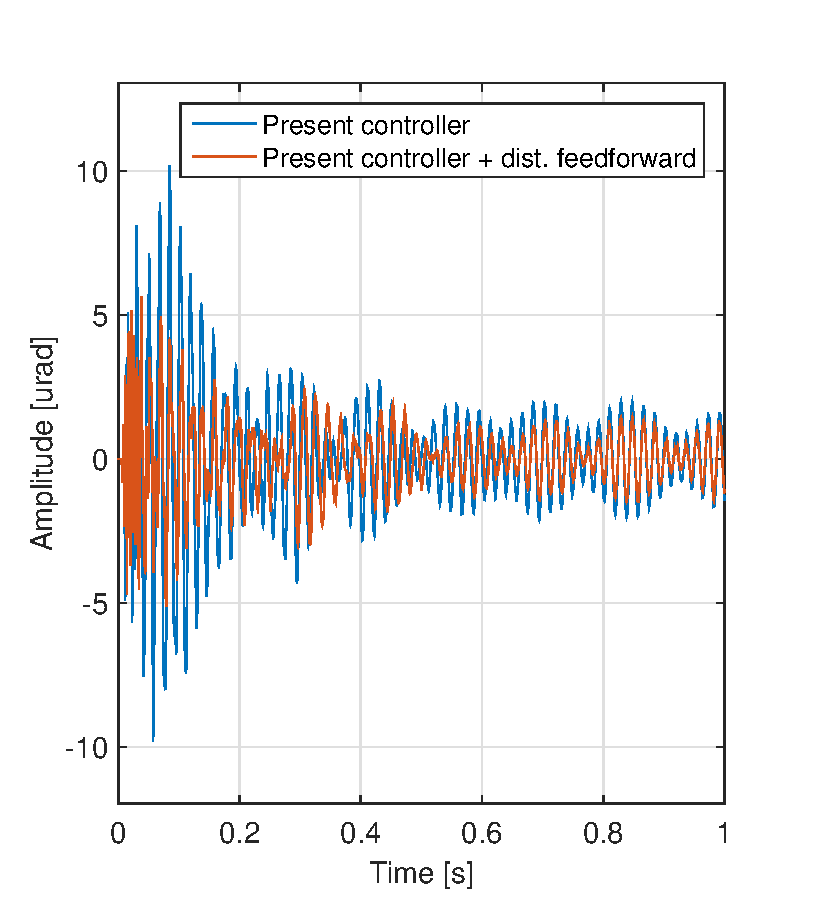
\includegraphics[width=0.43\textwidth, trim=0cm 0cm 1cm 0cm, clip=true]{../fig/matlab/cancellation_1_step_s.eps}}
    \qquad
    \subfloat[][Original acquired signal as disturbance ]{
    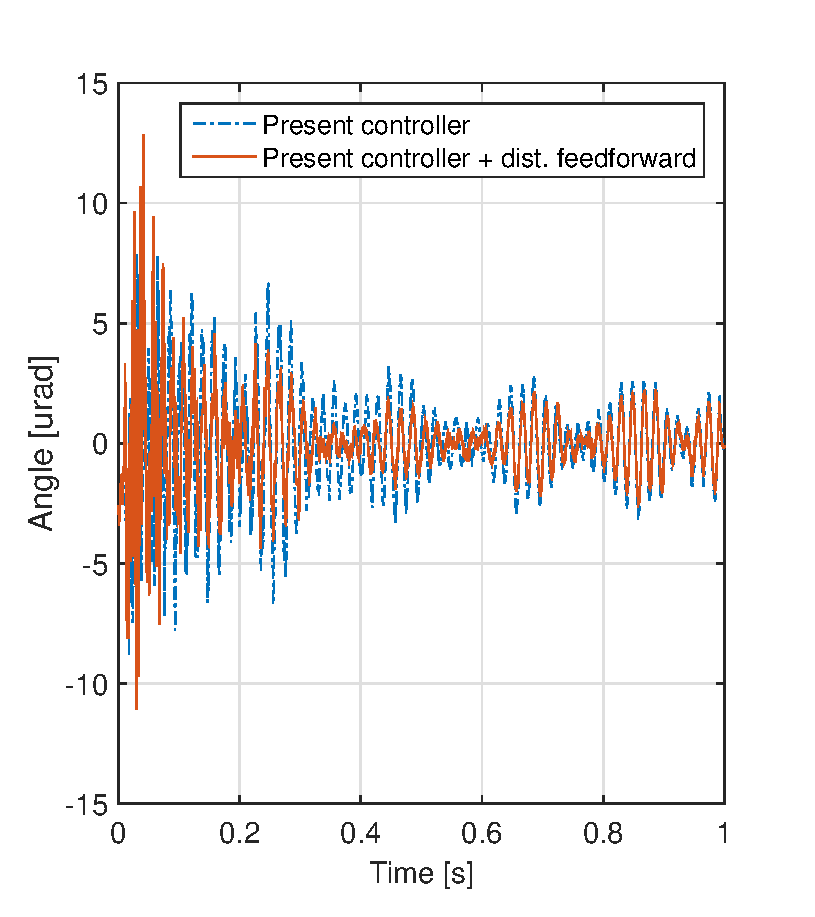
\includegraphics[width=0.43\textwidth, trim=0cm 0cm 1cm 0cm, clip=true]{../fig/matlab/cancellation_1_step_s_real_dist.eps}}
    %\caption{\label{fig:benchmark_dist} Feedforward disturbance cancellation with the mean of the acquired response added as disturbance (a) and one period of the acquired response added as disturbance (b). The disturbance cancellation is less effective with a slightly different disturbance.}
  \end{figure}
\end{frame}

\begin{frame}{Cancellation with Internal Model Principle}
  \alert{Idea}: Include a inverse model of the disturbance in the feedback loop to cancel the harmonic.
  \begin{itemize}
    \item Asymptotically reject the modeled disturbance
    \item Affecting the closed loop system
  \end{itemize}
\end{frame}

\begin{frame}{Cancellation with Internal Model Principle}
  \begin{figure}[h!]
    \centering %crop: left bottom right top
    \includegraphics[width=0.8\textwidth, trim=6.5cm 5.5cm 5.97cm 11cm, clip=true]{../fig/matlab/imp}
    %\caption{\label{fig:imp}Block diagram of the \abbrIMP control structure.}
  \end{figure}

  The generating polynomial $\Gamma(s) = f(0,s)/D(s)$.
  $C_{t}(s) = P(s)/(\Gamma(s)\bar{L}(s))$.
\end{frame}

\begin{frame}{Cancellation with Internal Model Principle}
  \begin{figure}[h!]
    \centering %crop: left bottom right top
    \subfloat[][Closed loop system]{
    \includegraphics[width=0.43\textwidth, trim=0cm 0cm 1cm 0cm, clip=true]{../fig/matlab/gc_imp.eps}}
    \qquad
    \subfloat[][Sensitivity function]{
    \includegraphics[width=0.43\textwidth, trim=0cm 0cm 1cm 0cm, clip=true]{../fig/matlab/s_imp.eps}}
    %\caption{\label{fig:rfdc_s_gc} Bode plot of the closed loop system shown in (a) and the sensitivity function (from output disturbance to system output) shown in (b) of the \abbrIMP and the present controller. The \abbrIMP is now attenuating disturbances at 50 Hz as seen in (b).}
  \end{figure}
\end{frame}

\begin{frame}{Cancellation with Internal Model Principle}
  \begin{figure}[h!]
    \centering %crop: left bottom right top
    \subfloat[][\label{fig:imp_model_error1}Attenuation of selected frequency]{
    \includegraphics[width=0.43\textwidth, trim=0cm 0cm 1cm 0cm, clip=true]{../fig/matlab/imp_model_error_real50.eps}}
    \qquad
    \subfloat[][\label{fig:imp_model_error2}Impact on 130 Hz component]{
    \includegraphics[width=0.43\textwidth, trim=0cm 0cm 1cm 0cm, clip=true]{../fig/matlab/imp_model_error_real.eps}}
    %\caption{\label{fig:imp_model_error}  Disturbance cancellation effectiveness with model errors. The attenuation of the major frequency is shown in (a) and the unwanted attenuation of the 130 Hz component is shown in (b).}
  \end{figure}
\end{frame}

\begin{frame}{Repetitive Feedforward Disturbance Cancellation}
  \begin{itemize}
    \item Cancellation of the 60, 90 and the 200 Hz
    \item Real acquired data used in simulations
    \item Not affecting other frequency components
  \end{itemize}
  \begin{figure}[h!]
    %\centering %crop: left bottom right top
    \subfloat[][]{
    \includegraphics[width=0.3\textwidth]{../fig/matlab/3_dist.eps}}
    \subfloat[][]{
    \includegraphics[width=0.3\textwidth]{../fig/matlab/3_dist_fft.eps}}
    \subfloat[][]{
    \includegraphics[width=0.45\textwidth]{../fig/matlab/3real_dist_fft.eps}}
  \end{figure}
\end{frame}

\begin{frame}{Repetitive Feedforward Disturbance Cancellation}
  \begin{figure}[h!]
    \centering %crop: left bottom right top
    \subfloat[][Time domain]{
    \includegraphics[width=0.43\textwidth, trim=0cm 0cm 1cm 0.8cm, clip=true]{../fig/matlab/model_conv.eps}}
    \qquad
    \subfloat[][FFT]{
    \includegraphics[width=0.43\textwidth, trim=0cm 0cm 1cm 0.8cm, clip=true]{../fig/matlab/model_conv_fft.eps}}
    %\caption{\label{fig:ph_lowgain} Observer convergence of the 200Hz harmonic with low gain, $G = [1, 0, 0, 0, 0, 0, 10, 0, 8, 0, 10, 0]^T$. The \abbrFFT of the time domain convergence (a) is presented in (b) which shows a good model of the 200 Hz harmonic.}
  \end{figure}
\end{frame}

\begin{frame}{Repetitive Feedforward Disturbance Cancellation}
  \begin{figure}[h!]
    \centering %crop: left bottom right top
    \subfloat[][Time domain]{
    \includegraphics[width=0.43\textwidth, trim=0cm 0cm 1cm 0.8cm, clip=true]{../fig/matlab/model_conv_w.eps}}
    \qquad
    \subfloat[][FFT]{
    \includegraphics[width=0.43\textwidth, trim=0cm 0cm 1cm 0.8cm, clip=true]{../fig/matlab/model_conv_fft_w.eps}}
    %\caption{\label{fig:ph_highgain} Observer convergence of the 200Hz harmonic with high gain, $G = [1, 0, 0, 0, 0, 0, 10, 0, 8, 0, 70, 0]^T$. The \abbrFFT of the time domain convergence (a) is presented in (b) which shows a less good model of the 200 Hz harmonic with a lot of other modeled frequency components in the region of 200 Hz.}
  \end{figure}
\end{frame}

\begin{frame}{Comparison}
  \scriptsize
  \begin{table}[h!]
    \centering
    \begin{tabular}{| l | P{3cm} | P{1.8cm} | P{1.8cm} | P{1.8cm} |}
      \hline
      \bf{No} & \bf{Aspect}  & \bf{Present} & \bf{IRC} & \bf{MRACPE} \\ \hline
      1 & Closed-loop Bandwidth [Hz] & 9.7 & 73.3 & -\\ \hline
      2 & Gain/Phase margin [dB / $^{\circ}$] & 14.4/66.2 & 13.1/49.4 & -\\ \hline
      3 & Tracking error, periodic input $\sigma$-[mrads] & $0.29$ & $0.03$ & $0.11$\\ \hline
      4 & Tracking error with model errors (model's 1st resonance at 22.0Hz), $\sigma$-[mrads] & $\infty$ & 0.03 & 0.21\\ \hline
      5 & Tracking error with model errors (model's 1st resonance at 67.2Hz), $\sigma$-[mrads] & $\infty$ & 0.03 & 0.11\\ \hline
      6 & Tracking error with model errors (model's 1st resonance at 17.6Hz), $\sigma$-[mrads] & $\infty$ & $\infty$ & 0.47\\ \hline
      7 & Tracking error with model errors (model's 1st resonance at 77.7Hz), $\sigma$-[mrads] & $\infty$ & $\infty$ & 0.11\\ \hline
    \end{tabular}
    %\caption{\label{tab:comp} Key parameters for the \abbrIRC, the \abbrMRACPE and the present control approach.}
  \end{table}
\end{frame}

\begin{frame}{Comparison}
  \scriptsize
  \begin{table}[h!]
    \centering
    \begin{tabular}{| l | P{3cm} | P{1.8cm} | P{1.8cm} | P{1.8cm} |}
      \hline
      \bf{No} & \bf{Aspect}  & \bf{Present} & \bf{IRC} & \bf{MRACPE} \\ \hline
      8 & Output disturbance rejection, settling time (1\%) [ms] & 8 & 25 & 260\\ \hline
      9 & Input/Output disturbance rejection, $\sigma$-[\unit{\micro\radian}] & $0.68 $/$1.43$ & $0.45$/$1.46$ & $1.95$/$1.41$\\ \hline
      10 & Stability issues & Unstable with high model errors & Unstable with high model errors, but better than present & Good adaption even with model errors, but tuning for quicker adaption easily leads to instability.  Stability only proven in continuous time. \\ \hline
      11 & Design and implementation considerations & Straight- forward technique, allowing for basic stability analysis & Same as present & Hard to tune. High computational burden for higher order models.\\ \hline
    \end{tabular}
    %\caption{\label{tab:comp} Key parameters for the \abbrIRC, the \abbrMRACPE and the present control approach.}
  \end{table}
\end{frame}

\begin{frame}{Comparison}
  \scriptsize
  \begin{table}[h!]
    \centering
    \begin{tabular}{| l | P{3cm} | P{1.8cm} | P{1.8cm} | P{1.8cm} |}
      \hline
        \bf{No} & \bf{Aspect} & \bf{FDC} & \bf{RFDC} & \bf{IMP} \\ \hline
      1 & Affecting closed loop system & No & No & Yes\\ \hline
      2 & Cancellation effectiveness of major frequency, attenuation-[\%]                & 64.6 & 88.4 & 83.3\\ \hline
      3 & Cancellation with model errors (model's 1st resonance at 28.2Hz), attenuation-[\%] & 40.5 & 26.6 & 73.5\\ \hline
      4 & Cancellation with model errors (model's 1st resonance at 43.4Hz), attenuation-[\%] & 57.7 & 5.0 & 83.4\\ \hline
      5 & Implementation considerations & Requires high order model, computational demanding. & Requires observer, computational demanding. Can be used as add-on.& Controller must be retuned when selecting a new frequency. \\ \hline
    \end{tabular}
    %\caption{\label{tab:comp_h} Key parameters for the harmonic cancellation methodologies.}
  \end{table}
\end{frame}

\begin{frame}[allowframebreaks]{References for Graphics}
  \bibliography{pres}
  \bibliographystyle{abbrv}
  All other references are listed in the Master's Thesis report.
\end{frame}

\end{document}
